\chapter{Problemløsning}
Mangler indledning o.O
\section{Kravspecifikationer}
I dette afsnit vil gruppen kigge og vurdere, hvilke krav der skal indegå i en løsning. Heri vil der både blive opstillet krav til en optimal løsning og til en afgrænset løsning, som gruppen mener at være realistisk, at kunne lave.

\subsection{Optimale løsningsforslag}
For at kunne udvilke en softwareløsning, der besvarer gruppens problemformulering, er det vigtigt at definere nogle krav til programmet. Til en optimal løsning, har gruppen vurderet, at der skal være følgende krav:
\begin{itemize}
	\item Programmet skal udvikles som en applikation til moderne smartphones, inklusiv iOS, Android og Windows. Phone. 
	\item Programmet skal vise et kort med ruten, og kortet skal vise attraktioner der er tæt på. 
	\item Programmet skal kunne beregne den korteste rute mellem en række punkter.
	\item Programmet skal vise rutevejledningen på samme måde som normale GPS-enheder. 
	\item Programmet skal give mulighed for at bedømme attraktioner, og derved tildele dem en rating, så de mest populære attraktioner kan findes. 
	\item Programmet skal give forslag til en anden rute, der inkludere attraktioner der ligger tæt på ruten.
	\item Programmet skal kunne  downloade en offline version af den rute der er valgt, inklusiv kortet for det omkringliggende område.
\end{itemize}
Til disse krav har gruppen konstrueret nogle skitser af den optimale løsning, for at give et billede af hvordan det eventuelt kunne se ud. \newline

\begin{wrapfigure}{r}{0.5\textwidth}
  \vspace{-20pt}
  \begin{center}
    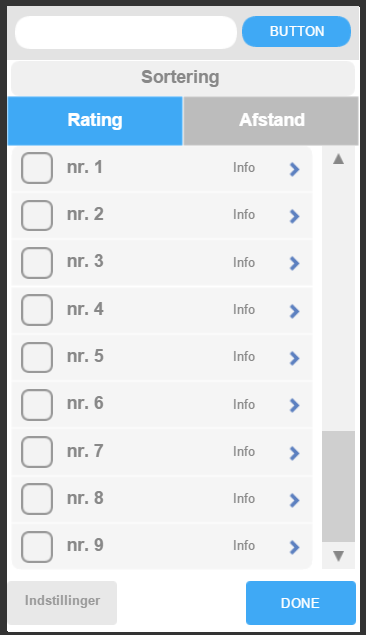
\includegraphics[scale=0.4]{start1} \newline
    \textit{Figur 3.1: Brugergrænseflade}\newline
  \end{center}
  \vspace{-20pt}
  \vspace{-10pt}
\end{wrapfigure}


Figur 3.1 viser den overordnede brugergrænseflade. Gruppen ønsker, at programmet skulle fungere på den måde, at der findes to valg muligheder, forholdsvis rating og afstand, hvoraf rating viser en række attraktioner med en værdi, baseret på hvad brugerne har valgt at rate den. Funktionen afstand, vil vise hvor stor en afstand der er fra det punkt hvor brugeren står, til en attraktion. De attraktioner, som brugeren ønsker at se, skal brugeren blot tjekke af, ved at klikke på attraktionerne (I dette tilfælde nr. 1, nr. 2 etc), og de vil derefter blive tilføjet til den nuværende rute. \newline

\begin{wrapfigure}{l}{0.5\textwidth}
  \vspace{-20pt}
  \begin{center}
    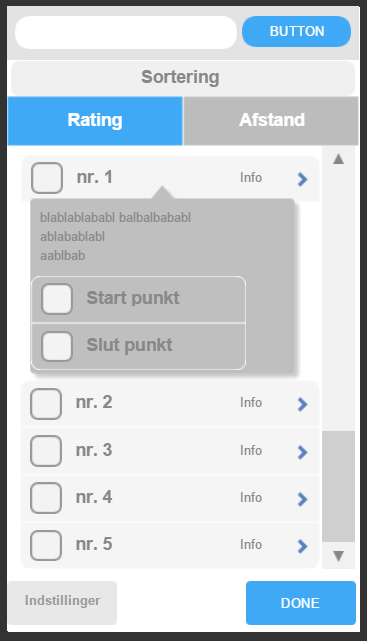
\includegraphics[scale=0.4]{start2} \newline
    \textit{Figur 3.2: Udvidet brugergrænseflade}\newline
  \end{center}
  \vspace{-20pt}
  \vspace{-10pt}
\end{wrapfigure}


Figur 3.2 viser en udvidet brugergrænseflade, hvor brugeren har valgt at klikke på drop-down-menuen "info". Denne menu vil derefter give bruger nogle informationer omkring attraktionen. Den vil derudover have to yderligere muligheder, start- og slutpunkt. Disse funktioner kan brugeren fx anvende, hvis der er en ønsket slut/start-lokalisation, hvor programmet derefter skal beregne den ønskede rute ud fra.\newline
\newpage

\begin{wrapfigure}{r}{0.5\textwidth}
  \vspace{-20pt}
  \begin{center}
    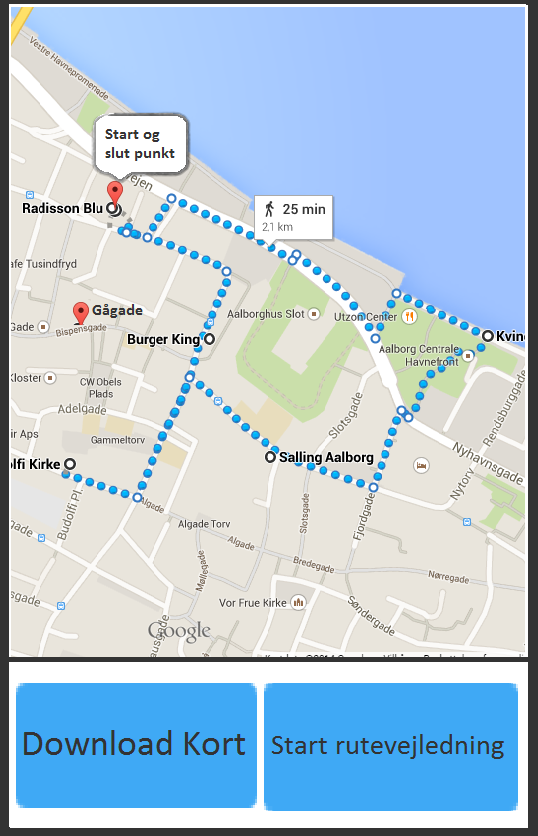
\includegraphics[scale=0.35]{rute1} \newline
    \textit{Figur 3.3: Ruten - Ruten er hentet fra Maps.Google.com}\newline
  \end{center}
  \vspace{-20pt}
  \vspace{-10pt}
\end{wrapfigure}

Figur 3.3 viser hvordan ruten fremvises, efter brugeren har valgt de attraktioner, som der ønskes at besøge. Ruten der vises, viser hvor lang hele ruten er, og hvor lang tid det tager at gå ruten. Herudover er der to knapper brugeren kan vælge at benytte sig af. Den ene knap er "download kort", som downloader kortet på mobilen, og derved gør det muligt at anvende programmet, uden at skulle bruge internet. Den anden knap "Start rutevejledning" viser vej og fortæller brugeren, hvornår han skal dreje etc. 
\newline
\newline
\newline
\newline
\newline
\newline

\begin{wrapfigure}{l}{0.5\textwidth}
  \vspace{-20pt}
  \begin{center}
    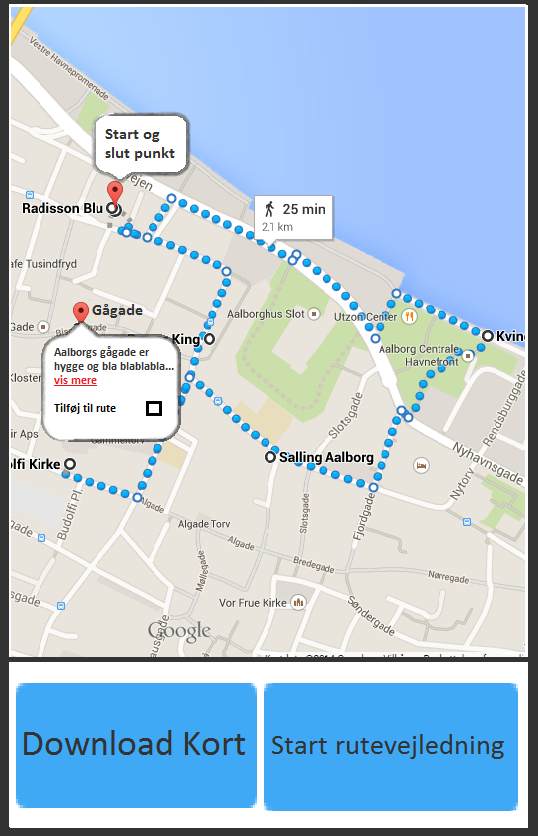
\includegraphics[scale=0.35]{rute2} \newline
    \textit{Figur 3.4: Udvidet rute - Ruten er hentet fra Maps.Google.com}\newline
  \end{center}
  \vspace{-20pt}
  \vspace{-10pt}
\end{wrapfigure}

Figur 3.4 er blot en udvidet version af den tidligere skitse. Forskellen på disse skitser er blot, at der i denne model, er vist hvordan der kan tilføjes flere punkter til den nuværende rute. Alle ikonerne på kortet, skal kunne klikkes på, hvor så der er mulighed for at tilføje disse punkter til ruten, hvis det ønskes, af brugeren. Herudover er der en "vis mere"-funktion, som vil vise informationer om attraktionen, brugeren har valgt, på samme måde som ved figur 2. \newline
\newline
\newline
\newline
\newline 

\subsection{Gruppens løsningsforslag}
Gruppen har gennem spørgskema og interview, fået stillet en række krav til løsningen, af turister og VisitAalborg. 
Gennem spørgskemaet, blev det konkluderet, at det vigtigste for turister, er at de kan opleve byen på en interessant rute. 
Derudover har turistbureauet givet udtryk for, at løsningen gerne skal være så enkelt som muligt, altså meget få funktioner, så brugeren ikke bliver forvirret, da de mener, at det er i turistens bedste interesse. \newline
Der er blevet stillet krav fra universitets side, om at programmet skal være et lille specifikt program i C, af høj kvalitet. Dette stemmer godt overens, med de krav der er blevet stillet fra turistbureauets side.   \newline
Ud fra dette, har gruppen opsat nogle krav for gruppens løsningsforslag, og de er som følgende:
\begin{itemize}
	\item Programmet skal kunne beregne den korteste rute mellem en række punkter.
	\item Programmet skal være i stand til at give forslag til en anden rute, der inkludere attraktioner der ligger tæt på ruten.
 	\item Programmet skal som output, give en liste over rutens destiationer, sorteret efter tiden til attraktionerne.
\end{itemize}

Da dette er et P1 projekt, og gruppen er begrænset af både tid og erfaring, har gruppen valgt at begrænse softwareløsningen, på følgende punkter: 
\begin{itemize}
	\item Rutevejledningen bliver i fugleflugtslinje.
	\item Brugeren kan kun vælge destinationer ud fra en række forudbestemte punkter.
	\item Tekstbaseret brugergrænseflade.
\end{itemize}

På baggrund af kravene og afgrænsningen, har gruppen tænkt sig at lave et program, som har nogle forudbestemte destinationer, der dækker over destinationerne i Aalborg, hvorefter brugeren vælger de destinationer han/hun ønsker at besøge. Programmet vil ud fra disse punkter, beregne den korteste rute, og undersøge om der er andre attraktioner, som ligger tæt på ruten, og spørge brugeren, om det kunne være interessant at besøge disse steder. Hvis ja, vil disse punkter også blive inkluderet. Resultatet bliver en liste over destinationerne, der står i rækkefølge, så turisten ved hvilken rækkefølge de skal besøge dem i, for at få den mest optimale rute.

\section{Teorier}
Indledning mangler.

\subsection{Grafteori}
Grafteori er et afsnit i denne rapport, som omhandler en generel forklaring på graf teori, hvorefter teorien bag ”Nærmeste Nabo Algoritme” vil blive beskrevet, herefter forklares ”udregningstid” i rute-algoritmer, og til sidst Traveling Salesman Problem. Alt dette beskrives, for at give et udgangspunkt for implementering af en hensigtsmæssig algoritme i programmet for denne rapport.\newline
Matematikken bag graf teori er ét aspekt af emnet, hvor visualisering og tegning er en anden. Den matematiske del behandler kombinationerne af knuder og kanter. En knude er et punkt, i vores tilfælde en attraktion som skal besøges, hvor en kant er vejen derhen. En kant er derfor længden fra ét punkt til det næste.
I graf teori er begrebet ”graf” mere fleksibelt, da punkterne ikke nødvendigvis har x, y eller z værdier, alt efter antallet af dimensioner man behandler det i. Grafen i denne form er en afbildning af punkter i den form, hvor det virker hensigtsmæssigt. Heraf opstår isomorfiske modeller, som er forskellige afbildninger, af selv samme graf. 

\begin{wrapfigure}{}{0.6\textwidth}
  \vspace{-45pt}
  \begin{center}
    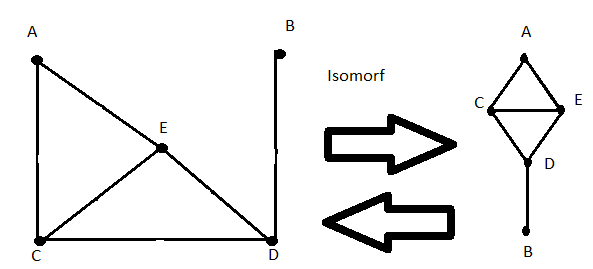
\includegraphics[scale=0.8]{grafteori1} \newline
    \textit{Figur 3.1: Brugergrænseflade}\newline
  \end{center}
  \vspace{-20pt}
\end{wrapfigure}

Denne matematik-type er stadig under udforskning, da der endnu ikke er en fuldstændig løsning på problemer i teorien, for blandt andet ”Traveling Salesman Problem”. Heriblandt findes mange typer af problemer, hvor forskellige teoretiske løsninger kan bruges. En af disse løsninger er den Nærmeste Nabo Algoritme (NNA, Nearest Neighbor Algorithm), som behandler et problem der opstår, når en række knuder skal indgå, og kun skal indgå én gang, hvilket betyder, at der ikke må være en løkke (loop). Dette opnåes gennem brug af Hamiltonian Paths, hvilket er en ”rute” gennem knuder på grafen. I NAA vil en kant have en værdi, og disse værdier er bestemmende for, hvilken kant der skal følges. Fra den knude der behandles, skal kanten med den laveste værdi følges. Dette kan dog optimeres, ved at lave en matrice over kanterne fra alle knuder. Her tages højde for hvilke kanter der samlet set giver den korteste rute, uden brug af løkker.

 
\begin{wrapfigure}{}{0.6\textwidth}
  \vspace{-45pt}
  \begin{center}
    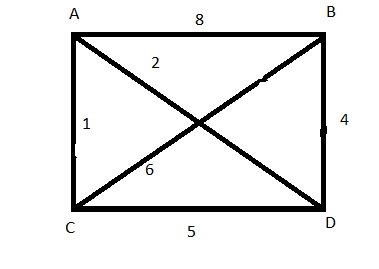
\includegraphics[scale=0.8]{grafteori2} \newline
    \textit{Figur 3.1: Brugergrænseflade}\newline
  \end{center}
  \vspace{-20pt}
\end{wrapfigure}

I dette tilfælde (figur 2), er den endelige rutes længde: 1+5+4+8 = 18. Spørgsmålet er så, er dette den koreste rute? Herefter opstilles en matrice, der beskriver alle kanter.
%TABULAR MANGLER%

\begin{tabular}{| l | l | l | l | l | l |}
	\hline
	  & A & B & C & D & E \\ \hline
	A & - & 3 & 1 & - & 2 \\ \hline
	B & 3 & - & - & 3 & 8 \\ \hline
	C & 1 & - & - & 5 & 6 \\ \hline
	D & - & 4 & 5 & - & 7 \\ \hline
	E & 2 & 8 & 6 & 7 & - \\
	\hline
	\end{tabular}


De mulige ruter er: \newline
ABDCE = 3+4+5+6 = 18. \newline
ACDBE = 1+5+4+8 = 18. \newline
AEBDC = 2+8+4+5 = 19. \newline
ABECD = 3+8+6+5 = 22. \newline
ABEDC = 3+8+7+5 = 23. \newline
ACEBD = 1+6+8+4 = 19. \newline
ACEDB = 1+6+7+4 = 18. \newline
AECDB = 2+6+5+4 = 17. \newline

Den korteste rute er altså AECDB, hvilket er 1 kortere end den antagede rute. Den optimale Hamiltonian Path er derfor denne rute. Dette tager NNA ikke højde for, da den starter i en valgt start-knude, og derefter følger kanten, med den derfra laveste værdi. Det smarte ved NNA er, at den ikke kræver meget kraft for en computer at udføre, hvorimod at finde den optimale Hamiltonian rute, vil være langt mere compliceret. NNA tager dog ikke højde for, hvad konsekvenser de skridt den tager, har for det endelige resultat.
Udover NNA, findes også Dijkstra’s algoritme, hvor første step er, at bestemme ende-knuden, og sætte dens distance til nul. Denne knude sættes til at være den første knude, som behandles. I det en knude er checket færdig, vil denne knude markeres som ”besøgt”, og kanten med den mindste værdi følges, og næste knude markeres som ”nuværende” knude. En kant bliver kun fulgt, hvis det er den korteste rute, tilregnet tidligere kanter.
Problematikken med Dijkstra’s algoritme i forhold til dette projekt er, at den checker den korteste rute fra start-knude til slut-knude, men den indkluderer ikke nødvendigvis alle knuder som oplyses. I det denne rapport er afgrænset til fugleflugtslinjer, vil Dijkstra’s ikke være den optimale. Hvis en rute igennem en by, hvor der er tilregnet veje, stier og andre knuder, vil Dijkstra’s være det bedste valg. Denne algoritme vil også være i brug ved den optimale løsning.
Ved brug af NAA vil en udregningstid for algoritmen beskrives som O(Nd), hvor N er kardinaliteten (antallet af knuder),  d er antallet af dimensioner, og O er udregningstiden. Dette vil sige, at for hver knude vi inddrager i udregningen, vil udregningstiden bliver antallet af dimensioner større. Denne udregningstid er baseret på, at udregningen bliver gjort gennem en ”naiv” metode, hvor udregningen konstant bliver testet for, hvorvidt den ”nuværende” beregnede rute, er kortere eller længere end den hurtigste hidtil.

\subsection{Matematikteori}
Essensen i dette projekt er at finde en flerpunktsrute mellem nogle valgte attraktioner, hvor brugeren skal have mulighed for, at vælge nogle attraktioner til deres rute. Gruppen vil ikke diktere hvad en interessant rute er for brugeren, derfor skal de have muligheden for at vælge de foreslåede attraktioner til eller fra.

\begin{wrapfigure}{}{0.4\textwidth}
  \vspace{-20pt}
  \begin{center}
    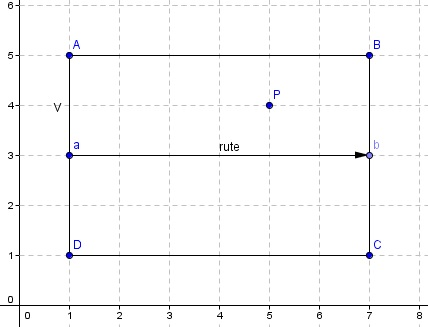
\includegraphics[scale=0.6]{matematikteori1} \newline
    \textit{Figur 3.1: Brugergrænseflade}\newline
  \end{center}
  \vspace{-20pt}
\end{wrapfigure}
 
Der tages nu udgangspunkt i figur X. En del af brugerens rute ligger fra attraktion a til attraktion b. Der skal nu tjekkes om der ligger andre attraktioner mellem afstanden fra a til b (eller AB), og med bredden AD hvor brugeren vil blive spurgt om denne attraktion skal tilføjes til ruten. AD er i projektets program sat til at være V * 2. Dette vil blive udregnet vha. vektorer 
Hvis der antages at punktet P er en attraktion som programmet skal tjekke, ligger denne inden for længden af ruten AB og bredden AD. Dette tjekkes med følgende formel:
\[0 < AP \cdot AB < AB \cdot AB \wedge 0 < AP \cdot AD < AD \cdot AD \]
Hvor prikproduktet af vektorerne AP og AB, skal være større end 0 og mindre end prikproduktet af vektorerne AB og AB. Det samme vil gælde for AD i stedet for AB.
Dog vil der først findes en vektor AP mellem punkterne A og P med formlen: \[ \overrightarrow{AP} = \begin{matrix}X2-X1 \\ Y2-Y1\end{matrix} \]
Vektor AP: A(1,5) og P(5,4): \[ \overrightarrow{AP} = \begin{matrix}5-1 \\ 4-5\end{matrix} = \begin{matrix} 4 \\ -1 \end{matrix} \]
\[ \text{Vektor AB er allerede kendt, da det er det samme som } \overrightarrow{ab} \text{.} \]
For at projektere AP på AB skal følgende formel benyttes: \[ b_{a} = (\frac{a*b}{|a|^2}) * a \]
Med denne formel vil vektoren b blive projekteret på vektoren a. I tælleren findes prikproduktet som kan findes ved at: \[ a \cdot b = \begin{matrix}X1 * X2 \\ Y1 * Y2\end{matrix}  \]
I nævneren findes længden på vektor a i anden, som kan regnes ved at sige: \[ \sqrt{ax^2+ay^2}^2 \]
Hvis der forsat kigges på eksemplet med figur X, vil projektionen af AP på AB se således ud:
Prikproduktet af vektorerne: \[ \overrightarrow{AP} \cdot \overrightarrow{AB} = \begin{matrix} 4 & 6 \\ -1 & 0 \end{matrix} = 4*6+(-1)*0 = 24 \]
Længden af AB vil være: \[ \sqrt{6^2+0^2}^2 = 36 \]
Ud fra dette kan vektoren fra projektionen af AP på AB findes: 
\[ \frac{24}{36} * \begin{matrix} 6 \\ 0 \end{matrix} \rightarrow \frac{24}{36} * 6 \wedge \frac{24}{36} * 0 = \begin{matrix} 4 \\ 0 \end{matrix} \]

\begin{wrapfigure}{R}{0.4\textwidth}
  \vspace{-60pt}
  \begin{center}
    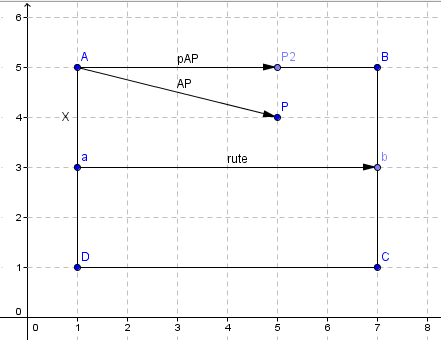
\includegraphics[scale=0.6]{matematikteori2} \newline
    \textit{Figur 3.1: Brugergrænseflade}\newline
  \end{center}
  \vspace{-60pt}
\end{wrapfigure}

Hvor resultatet vil give en ny vektor: \[ \begin{matrix} 4 \\ 0 \end{matrix} \text{ ,} \]  som også vil have startpunkt i A. Hvis der igen kigges på formlen:
\[0 < AP \cdot AB < AB \cdot AB \wedge 0 < AP \cdot AD < AD \cdot AD \]
overholder punktet P første del, og ovenstående metode skal derfor gentages med vektoren AD i stedet for AB, for matematisk at finde ud af om punktet ligger inden 	for den afsatte bredde og længden af ruten a til b. Ved udregning af projektionen af AP på AD vil den nye vektor hedde: \[ \begin{matrix} 0 \\ -1 \end{matrix} \text{ .} \]


\section{Implementering}
I dette afsnit vil programmet blive beskrevet, både en overordnet programbeskrivelse og en dybdegående forklaring af programmets funktioner. Derudover vil der blive beskrevet hvordan brugeren interagere med programmet. 

\subsection{Programbeskrivelse}
Programmet begynder med at indlæse alle de forudbestemte tilgængelige attraktioner fra en tekstfil. Alle disse attraktioner bliver vist på en liste for brugeren i kommandopromten med numre ud for hver attraktion. Brugeren vælger så hvilke attraktioner vedkommende har lyst til at besøge, ved at indtaste attraktionens nummer, hvor attraktionen så vil blive tilføjet til en liste. Denne liste kører gennem programmet, og den korteste rute bestemmes. Programmet tjekker derefter, for nærliggende attraktioner der kan tilføjes til ruten, på samme måde som i begyndelsen da de valgte attraktioner til deres rute. Hvis brugeren vælger ekstra attraktioner til deres rute, kører programmet igen, og den nye rute beregnes. Når ruten er beregnet, vil ruten være tilgængelig i tekstfilen ”KortesteRute.txt”, hvor brugeren kan se hvilken rækkefølge attraktionerne skal besøges i, og distancen mellem dem. 

Attraktionerne til programmet bliver indlæst fra en .txt fil når prorammet køres. I programmet bliver filen indlæst i en funktion som hedder initialiserAttraktioner. Hvis filen ikke er tom vil elementerne, vha. funktionen fscanf, blive indlæst i grupper af 4, hvor de bliver indlæst som ”attraktion” hvilket er defineret som et struct. Hvis filen er tom, vil en advarsel blive vist i prompten og lukke programmet ned. Når alt information er indlæst fra filen, og den ikke længere er nødvendig, lukkes filen.
Indsæt billede af ”initialiserAttraktioner”.
Brugeren bliver præsenteret for en liste over alle tilgængelige attraktioner fra inputparameteren, og attraktionernes tilhørende nummer i funktionen ” valgafAttraktioner”. Brugeren bliver bedt om at indtaste attraktionernes matchende numre, hvilket vil blive tilføjet til en liste. Taster brugeren 0, bliver brugeren præsenteret for sine valg, og beregningen af den korteste rute igangsættes. Programmet returnere listen af valgte attraktioner.
Indsæt billede af ” valgafAttraktioner”.	
Funktionen ”findNaboRute” benytter NNA (Nearest Neighbour Algorithm, eller Nærmeste Nabo Algoritme), til at finde den korteste rute mellem en række attraktioner for et bestemt startsted, der er opgivet i inputparametrene. Efter at have fundet den korteste rute ud fra NNA som en beskrevet i teoriafsnittet X, returnere den et array med ruten og distancen for denne rute. 
Indsæt billede af ”findNaboRute”.
”findKortesteNaboRute” benytter funktionen ”findNaboRute”, til at finde ud af hvilket startsted der giver den korteste rute. Dette gøres ved at sætte en variable til en stor værdi, som rutedistancen ikke vil gå over, og opdatere den hvis ”findNaboRute” returnere en distance for de givne attraktioner med en given start attraktion, der er lavere end de forgående ruter. ”findKortesteNaboRute” returnere et array der er en sorteret liste over attraktionerne, og den samlede længde mellem disse. 
Indsæt billede af ”findKortesteNaboRute”. \newline
Funktionen ”beregn\_dist” er en implementering af Harasin formlen, der er beskrevet i teoriafsnittet X. Funktionen tager længde- og breddegrader for to attraktioner som inputparametre. Disse længde- og breddegrader bliver brugt i formlen til at udregne distancen mellem de to punkter. Funktionen returnere til sidst den beregnede distance mellem de to attraktioner.
Indsæt billede af ”beregn\_dist”.
Funktionen ”udregn\_kanter” bruges til at udregne distancen mellem punkterne. Beregningen af distancerne sker vha. ”beregn\_dist”, ved at sende længde- og breddegrader for attraktionerne, og opretter en kant. Dette gøres i en for løkke i en anden for løkke, hvor der for hvert punkt blive udregnet distancen til de punkter der ikke allerede er blevet oprettet en kant for i en tidligere itteration af løkkerne. Kanterne bliver tilføjet til kantarrayet, gennem den pointer der er inputparameter til funktionen, så kanterne kan blive tilgået fra resten af programmet. 
Indsæt billede af ”udregn\_kanter”.
Brugeren af programmet bliver præsenteret for ruten gennem funktionen ”output\_liste”. Funktionen udskriver en liste med attraktionerne i den rækkefølge de skal besøges, hvis den korteste rute ønskes. Funktionen sørger også for at skrive distancen mellem attraktionerne. 
Indsæt billede af ”output\_liste”.
BESKRIV FUNKTIONEN ”findDist”.

\subsection{Opsummering}
Her er en liste med de overstående funktioner, med en kort forklaring om hvad hver funktions opgave i programmet er.
\begin{itemize}
	\item "InitialiserAttraktioner" – Initialisere attraktioner fra en tekstfil
	\item "valgafAttraktioner" – Lader brugeren vælge attraktioner
	\item "findNaboRute" – Bestemmer den korteste rute mellem en række attraktioner, for en bestemt attraktion
	\item "findKortesteNaboRute" – Finder det optimale startsted
	\item "beregn\_dist" – Beregner distancen mellem to attraktioner
	\item "udregn\_kanter" – Bruger ”beregn\_dist” til at oprette kanter mellem attraktioner
	\item "output\_liste" – Udskriver den korteste rute til brugeren
	\item "findDist" - ..
\end{itemize}


